%%%%%%%%%%%%%%%%%%%%%%%%%%%%%%%%%%%%%%%%%%%%%%%%%%%%%%%%%%%%%%%%%%%
% Background
% Team:
% Wolverine
% Members: 
% Dexter Chen, Eric Chang, Eric Lee, Jacky Wu, Karthick Mani, Kenvin Lo, Yu-cheng Chen
% Relative files:
% Main.tex, Background_Wolverine.tex, Library.bib, Wolverine_Background_Chart_1.png
% Note: 
% Do not compile this file compile Main.tex to get the pdf file instead.
%%%%%%%%%%%%%%%%%%%%%%%%%%%%%%%%%%%%%%%%%%%%%%%%%%%%%%%%%%%%%%%%%%%
	
\subsection{Information retrieval on existing database}
\textit{\footnotesize Author:Dexter Chen, Eric Chang, Eric Lee, Jacky Wu, Karthick Mani, Kenvin Lo, Yu-cheng Chen.}\\

We live in the time where technologies evolve beyond our imagination. Due to the rapidly increasing amount of information, we can't rely on the old fashion ways to find data. We need new information retrieval methods to handle such a big amount of data. But most of the information retrieval methods such as search engine can't really search everything on the web. They can only search the data that has been captured into the database according to \cite{Grehan2002}. Thus, we need to create a database to store these data and automatically update them frequently.

There are several online libraries currently available for us to get the academic articles we need. And they can be roughly divided into three group according to the way they store articles.

\paragraph{Index libraries}
	These kind of libraries stores the index and abstract of the articles. They don't provide the full-text documents directly, but may give the linkage to the publisher websites of articles. And can be categorized by the type of articles they include.
	\begin{itemize}
		\item\textbf{Comprehensive topics}\\Libraries such as Web of Science, Scopus...
		\item\textbf{Specialized topics}\\Libraries such as Compendex, BIOSIS Previews, PubMed...
	\end{itemize}
	
\paragraph{Publisher libraries}
	These libraries are created by the publishers themselves, so they provide the newest and complete documents directly. And can also be categorize by the type of articles they include.
	\begin{itemize}
		\item\textbf{Comprehensive topics}\\Libraries such as Science Direct, Springer Link, Wiley Online Library...
		\item\textbf{Specialized topics}\\Libraries such as Nature.com, Emerald Management Xtra, IEEE Xplore...
	\end{itemize}
	
\paragraph{Aggregator libraries}
	These libraries do not publish the articles by themselves, but they still sometimes provide the full-text articles to the user. The way they do this is to negotiate with some of the publisher libraries and get the authorization of the articles. Libraries such as EBSCOhost, ProQuest, JSTOR...

\subsubsection{Introduction to several libraries }
\begin{enumerate}
	\item\textbf{PubMed}
	\setlength{\parindent}{2em}
		
	 PubMed is a free library which is used for searching reference papers and abstracts related to the biomedical topics. PubMed’s design philosophy is based on full-text XML files, which are readable by both the machines, humans and moreover technology independent. PubMed is classified into Index libraries, which is the prime reason that it won’t be able to provide full text in some papers. For the type of database used by PubMed is Microsoft SQL server, which is a relational database to store all of the archives such as XML, images, PDF files supplementary, etc.
	
	%\item\textbf{Science Direct}
	%\item\textbf{Springer Link}
	
	\item\textbf{IEEE Xplore}
	\setlength{\parindent}{2em}
	
	IEEE Xplore is a scholarly research library formerly known as IEEE/IET Electronic Library (IEL). The IEEE is an acronym for Institute of Electrical and Electronics Engineers, which is one of the leading standard organizations in the world. More than 3.5-million full-text documents in the field of electrical, engineering, computer science and electronics are provided in this library. 
	
	The front and user interface of IEEE library present the information on the screen, including the latest Angular, Jquery, HTML 5, CSS, etc. Most of the HTML for PDF, either it is for journal (conference) articles or standards get dynamic transformations real time and served through MarkLogic. Endeca, which is an Oracle product powers Xplore searches, is used in the search layer. All PDF files are fed through Endeca system. Endeca servers will provide the matching documents and Xplore platform presents it on the screen to the user. And all the content is stored in oracle metadata which will be consumed by Endeca, MarkLogic Authentication, and Authorization services.
	
\end{enumerate}

\begin{figure*}[htb]
	\begin{center}
		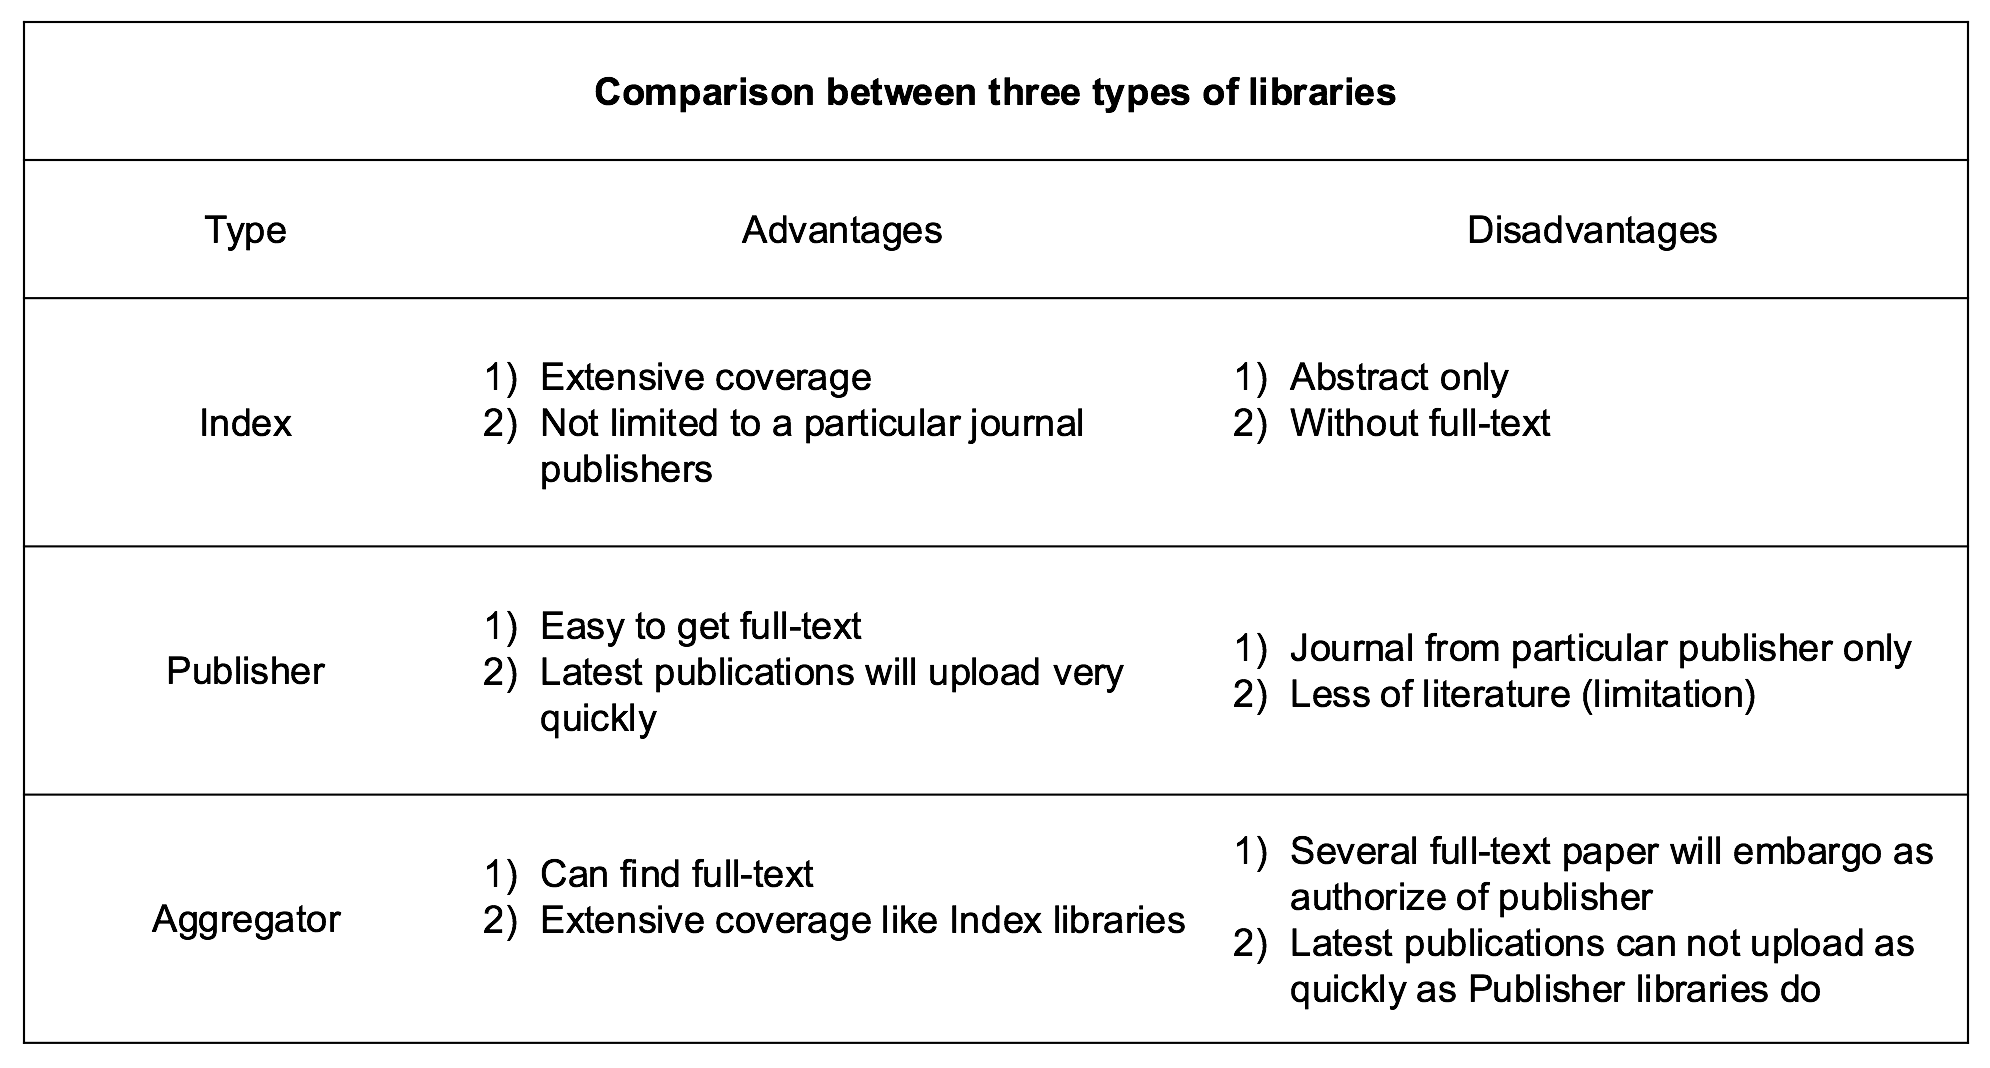
\includegraphics[width=0.8\textwidth]{Wolverine_Background_Chart_1}
	\end{center}
	\caption{Comparison between three types of libraries}
\end{figure*}
\newpage
